\subsection{Stima teorica dell'accettanza del rivelatore}
  In questa sezione, come suggerito dal titolo, si procederà con il calcolo della stima teorica dell'accettanza del sistema di acquisizione nelle due configurazioni usate 
  nell'esperienza. Tali stime verranno effettuate usando fondamentalmente 2 ipotesi, più una aggiuntiva per il caso del decadimento a 3 fotoni. Le 2 ipotesi comuni consistono 
  nell'assumere che il decadimento avvenga al centro di una sfera di raggio \(R\) sulla cui superficie sono situati i rivelatori di raggio \(r\) e nel considerare il rapporto 
  \( \frac{r}{R} << 1 \) in maniera tale che \(\arctan\left(\ \frac{r}{R} \right) \approx \frac{r}{R} \). Quest'ultima ipotesi implica che i rivelatori, che verranno rappresentati come
  circonferenze, sono equivalentemente rappresentati da cerchi sulla superficie sferica e viceversa. Partiamo quindi dal caso più semplice. La stima fatta vuole
discutere l'angolo solido in senso lato coperto dai rivelatori rispetto all'evento analizzato, e non si prefigge di studiare la possibilità che il fotone non
interagisca con il rivelatore.
  \subsubsection{Decadimento a due corpi, rivelatori a 180 gradi}
  Avendo a che fare con un decadimento a due corpi con momento iniziale nullo i due fotoni emessi avranno momento uguale ed opposto e di conseguenza, posizionando due rivelatori
  a \(180^\circ\), se un fotone colpisce un rivelatore automaticamente l'altro interagirà con il secondo rivelatore facendo si che l'evento venga effettivamente rivelato. La
  probabilità che un generico decadimento a 2 fotoni venga rivelato corrisponde alla probabilità che un fotone interagisca con  uno dei due rivelatori, pari al rapporto tra la 
  somma tra le aree dei due rivelatori e la superficie della sfera di raggio R, essendo per isotropia la probabilità di emissione uguale per tutte le direzioni. Quindi
  \(P\left(2\gamma\right) = \frac{r^2}{2R^2}\).
  \subsubsection{Decadimento a tre corpi, rivelatori a 120 gradi}
  Il caso del decadimeto a tre fotoni è molto più delicato, essendo un decadimento a tre corpi lo spettro dell'energia è continuo e dipende dall'angolo di emissione. Ciò che però
  si può dire è che i tre fotoni vengono emessi complanari, per effetto sempre della conservazione del momento lineare. In questo caso i tre scintillatori vengono posti a \(120^\circ\)
  l'uno dall'altro sullo stesso piano. Introduciamo a questo punto una nuova ipotesi al fine di semplificare il cacolo, ovvero che anche i tre fotoni vengano emessi ad un angolo di
  \(120^\circ\) l'uno dall'altro, cosicchè se due fotoni interagiscono con due rivelatori anche il terzo interagirà con l'ultimo rivelatore. 
  
  Al fine di calcolare la probabilità che un evento venga rivelto conviene fissare un sistema di riferimento con origine nel centro della sfera di raggio R
  e con asse \(z\) che passa per il centro del rivelatore interagente con il primo fotone. Gli altri due assi si scelgono in maniera tale che i centri degli altri due rivelatori
  giacciano sul piano \(xz\).\\
  
  \begin{figure}[h]\centering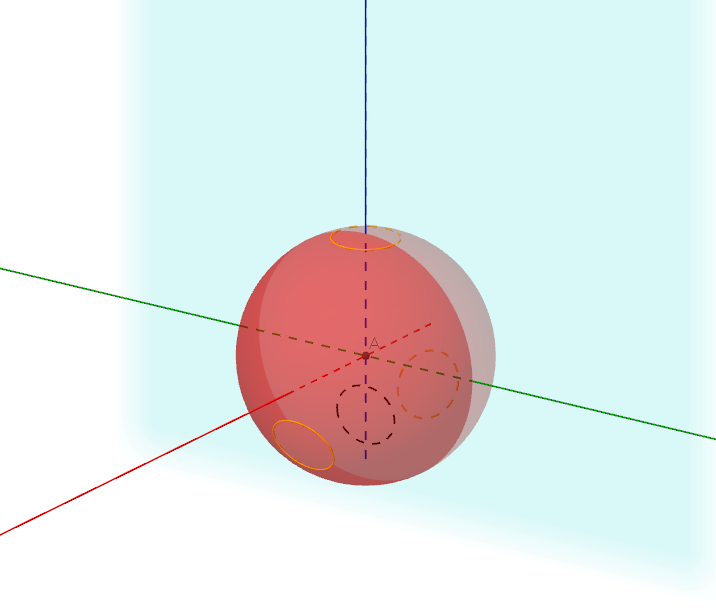
\includegraphics[width=0.9\textwidth]{../../img/sfera_sdr.png}\caption{Collocazione dei rivelatori nel sistema di riferimento scelto. }\label{fig:sfera_sdr}\end{figure}


  Il passo successivo consiste nel parametrizzare le traiettorie dei singoli fotoni. \'E necessario parametrizzarne soltanto due, poichè il terzo interagisce automaticamente con il
  sistema di acquisizione una volta che i primi due lo hanno fatto. E' molto comodo utilizzare le coordinate sferico polari, in maniera tale che la traiettoria del primo fotone sia 
  nella direzione del versore \(n_1 = \left( \cos \phi \sin \theta , \sin \phi \sin \theta, \cos \theta  \right)\) con \(\theta\) angolo azimutale, e similmente per il secondo fotone
  \(n_2 = \left( \cos \alpha \sin \beta , \sin \alpha \sin \beta, \cos \beta  \right)\) con questa volta \(\beta\) come angolo azimutale. Poichè per ipotesi il primo fotone
  interagisce con il rivelatore posto al polo \(\left(0,0,R \right)\), l'angolo \(\theta\) è vincolato ad essere minore di \(\arctan\left(\ \frac{r}{R} \right) \approx \frac{r}{R} << 1 \)
  e di conseguenza \(\sin \theta \approx \theta \) e \(\cos \theta \approx 1 \). Si userà questo risultato a breve. A questo punto bisogna imporre che l'angolo tra i due versori sopra 
  definiti sia di \(120^\circ\), ovvero \(n_1 \cdot n_2 = \cos (120^\circ) = -\frac{1}{2}\). Questa condizione si traduce nell'espressione \[\sin \theta \sin \beta \left( \cos \phi \cos \alpha
  + \sin \phi \sin \alpha \right) + \cos \theta \cos \beta = \mu \sin \theta \sin \beta  + \cos \theta \cos \beta =-\frac{1}{2}\] con \(\mu := \left( \cos \phi \cos \alpha + 
  \sin \phi \sin \alpha \right) = \cos \left( \alpha - \phi \right) \). Al fine di risolvere tale equazione si ricorre alla sopracitata approsimazione, ottenendo quindi 
  \( \mu \theta \sin \beta + \cos \beta = -\frac{1}{2}\), risolvibile utilizzando l'identita fondamentale della trigonmetria \(\sin \beta = \pm \sqrt{1 - \cos^2 \beta}\), per cui
  \(\mu^2 \theta^2 \left( \sqrt{ 1 - \cos^2 \beta } \right)^2 = \left( -\frac{1}{2} - \cos \beta \right)^2  \) ed usando la variabile ausiliaria \(t = \cos \beta\) ci si riconduce 
  a risolvere l'equazione \(t^2 \left( 1 + \mu^2 \theta^2 \right) + t + \frac{1}{4} - \mu^2 \theta^2=0\) che ha come soluzioni :
  $$ t_{1,2} = \frac{-1 \pm \mu \theta \sqrt{3} \sqrt{1 + \frac{4}{3} \mu^2 \theta^2 }}{2\left( 1 + \mu^2 \theta^2 \right)} \approx$$
  $$ \frac{1}{2}\left(-1 \pm \mu \theta \sqrt{3} \left(1 + \frac{2}{3} \mu^2 \theta^2 \right)\right)\left( 1 - \mu^2 \theta^2 \right) \approx \frac{1}{2} \left( -1 \pm \mu \theta \sqrt{3} \right)$$
  dove si sono trascurati gli ordini superiori al primo in \(\theta\) poichè quest'ultimo è piccolo per ipotesi. Per decidere quale tra i due segni prendere si pensi di porsi a
  \( \phi = \alpha \) per cui \(\cos \left( \phi - \alpha \right) = 1\), ad un aumento di \(\theta\) deve corrispondere un aumento di \(\beta\), ovvero una diminuzione del \(\cos \beta\),
  quindi in definitiva: \(t= \cos \beta \approx -\frac{1}{2} \left( 1 + \mu \theta \sqrt{3} \right) \).
  A questo punto si cerchi la condizione per cui il secondo fotone interagisca con uno dei due rivelatori rimanenti, supponiamo questo sia quello con centro nel terzo quadrante
  del piano \(xz\). La proiezione di quest'ultimo sul piano \(yz\) è un'ellisse di centro \(\left(0,0,-R \sin 30^\circ \right)\), asse maggiore parallelo all'asse \(y\) di lunghezza \(r\) e asse minore invece parallelo
  all'asse \(z\) di lunghezza \(r \cos 30^\circ\). L'equazione di questa ellisse sul piano \(yz\) è:
  $$ \frac{y^2}{r^2} + \frac{\left( z + R \sin 30^\circ \right)^2}{\left(r \cos 30^\circ\right)^2} = 1 = \frac{1}{r^2}\left(y^2 + \frac{4}{3} \left( z + \frac{R}{2} \right)^2 \right) $$
  
  \begin{tikzpicture}
\draw[->,thick] (-5,0)--(5,0) node[right]{$y$};
\draw[->,thick] (0,-5)--(0,5) node[above]{$z$};

\draw(0,0) circle(4);
\draw(-1.5,-2)--(1.5,-2);
\draw(0,-2) ellipse[x radius = 1.5,y radius = 1];

\node [label=below right:-R/2,draw,fill=black,circle,inner sep=0pt,minimum size=3pt] at (0,-2) {};
\draw[decorate, decoration={brace, mirror}] (-1.5,-2.1) -- (0,-2.1);
\draw[decorate, decoration=brace] (-0.1,-2) -- (-0.1,-1);

\node [label= left :$r \cos 30$] at (-0.11,-1.5) {};
\node [label= below :$r$] at (-0.75,-2.11) {};
\node [label= above right :$R$] at (4,0) {};

%\node [label=below right:B,draw,fill=black,circle,inner sep=0pt,minimum size=3pt] at (1.5,0) {};
%\node [label=above right:C,draw,fill=black,circle,inner sep=0pt,minimum size=3pt] at (0,1) {};
%\node [label=below:F,draw,fill=black,circle,inner sep=0pt,minimum size=3pt] at (-0.87,0) {};
%\node [label=below:F',draw,fill=black,circle,inner sep=0pt,minimum size=3pt] at (0.87,0) {};
%\node [label=below left:-R/2,draw,fill=black,circle,inner sep=0pt,minimum size=3pt] at (-4,0) {};
\end{tikzpicture}
  
  Si noti che se le coordinate \(x\) e \(y\) appartenenti al vettore \(R n_2 = \left( x, y, z \right)\) che parametrizza l'intersezione tra la traiettoria del secondo fotone e la 
  superficie sferica di raggio \(R\) sono interne all'ellisse, allora il fotone ha interagito con il rivelatore. Prima di procedere calcoliamo il \(\sin \beta \) in funzione di $\theta$ in base a
  ciò che sappiamo di \(\cos \beta\). Infatti: 
  $$ \sin \beta = \pm \sqrt{1 - \cos^2 \beta} \approx \pm \sqrt{1 + \frac{1}{4} \left( 1 + \mu \theta \sqrt{3} \right)^2 } = \pm \sqrt{\frac{3}{4} - \frac{\sqrt{3}}{2} \mu \theta - \frac{3}{4} \mu^2 \theta^2 }  $$
  Poichè \(0 \le \beta \le \pi\), allora \(\sin \beta \ge 0\), si prenderà il segno \(+\) nell'equazione sopra. Inoltre si trascurano nuovamente i termini del secondo ordine in \(\theta\).
  Quindi:
  $$ \sin \beta \approx \frac{\sqrt{3}}{2} \sqrt {1 - \frac{2}{\sqrt{3}} \mu \theta} \approx \frac{\sqrt{3}}{2} \left(1 - \frac{1}{\sqrt{3}} \mu \theta \right)  $$
  di nuovo nell'ultimo passaggio si è usata l'ipotesi di \(\theta\) piccolo, condizione che impedisce al radicando della espressione sopra di diventare negativo.
  Con questo risultato si può efficacemente parametrizzare \(R n_2 = R \left( \cos \alpha \sin \beta , \sin \alpha \sin \beta, \cos \beta  \right) = 
  R \left( \frac{\sqrt{3}}{2} \left(1 - \frac{1}{\sqrt{3}} \mu \theta \right) \cos \alpha , \frac{\sqrt{3}}{2} \left(1 - \frac{1}{\sqrt{3}} \mu \theta \right) \sin \alpha ,
  -\frac{1}{2} \left( 1 + \mu \theta \sqrt{3} \right) \right)\), ed imponendo che \(y^2 + \frac{4}{3} \left( z + \frac{R}{2} \right)^2 \le r^2 \) si ottiene:
  $$ \frac{r^2}{R^2} \ge \frac{3}{4} \left(1 - \frac{1}{\sqrt{3}} \mu \theta \right)^2 \sin^2 \alpha + \frac{4}{3} \left( -\frac{1}{2} \left( 1 + \mu \theta \sqrt{3} \right) + \frac{1}{2} \right)^2 \approx  $$
  $$ \frac{3}{4} \left(1 - \frac{2}{\sqrt{3}} \mu \theta + \frac{1}{3} \mu^2 \theta^2 \right)\sin^2\alpha + \mu^2 \theta^2 $$
  trascurando nuovamente i termini del secondo ordine si giunge alla seguente:
  $$ \frac{3}{4} \left(1 - \frac{2}{\sqrt{3}} \mu \theta \right)\sin^2\alpha \le \frac{r^2}{R^2} $$
  ovvero
  $$ \sin^2\alpha \le \frac{4r^2}{3R^2} \frac{1}{1 - \frac{2}{\sqrt{3}} \mu \theta} \approx \frac{4r^2}{3R^2} \left(1 + \frac{2}{\sqrt{3}} \mu \theta \right)  $$
  Si noti che l'espressione \(1 - \frac{2}{\sqrt{3}} \mu \theta \ge 0\) per le ipotesi fatte su \(\theta\).\\
  Per ricavare una condizione su \(\alpha\) bisogna ora fare un'ulteriore osservazione. Da considerazioni legate alla geometria del problema, si nota che l'angolo \(\alpha\) è anch'esso
  minore in modulo di \(\arctan\left( \frac{r}{R} \right)\) e può essere quindi considerato piccolo. Di conseguenza \(\mu = \cos \phi \cos \alpha + \sin \phi \sin \alpha = \cos \phi + \alpha \sin \phi \)
  e \(\sin^2 \alpha \approx \alpha^2\). La condizione qui sopra può quindi essere riscritta:
  $$ \alpha^2 \le  \frac{4r^2}{3R^2} \left(1 + \frac{2\theta}{\sqrt{3}} \left( \cos \phi + \alpha \sin \phi \right)  \right)  \to $$
  $$ \alpha^2 -\frac{8r^2\theta}{3\sqrt{3}R^2}\sin \phi \alpha -\frac{4r^2}{3R^2}\left( 1 +\frac{2 \theta}{\sqrt{3}} \cos \phi \right) \le 0 $$
  risolviamo l'equazone di secondo grado associata alla disequazione appena ricavata.
  $$ \alpha_{1,2} = \frac{8r^2\theta}{3\sqrt{3}R^2}\sin \phi \pm \sqrt{ \left( \frac{8r^2\theta}{3\sqrt{3}R^2}\sin \phi \right)^2 + \frac{16r^2}{3R^2}\left( 1 +\frac{2 \theta}{\sqrt{3}} \cos \phi \right)} \approx $$
  $$ \frac{8r^2\theta}{3\sqrt{3}R^2}\sin \phi \pm \frac{4r}{\sqrt{3}R}\sqrt{ 1 +\frac{2 \theta}{\sqrt{3}} \cos \phi} \approx \frac{8r^2\theta}{3\sqrt{3}R^2}\sin \phi \pm \frac{4r}{\sqrt{3}R}\left( 1 +\frac{\theta}{\sqrt{3}} \cos \phi \right) =: A \pm B$$
  Di conseguenza la precedente disequazione è soddisfatta per \(A-B\le \alpha \le A + B\).\\
  L'ultimo passo per determinare la probabilità che il secondo fotone interagisca con uno dei due rivelatori consiste nel notare che tale probabilità è equivalente a quella
  che lo stesso fotone interagisca con un solo rivelatore ed imponendo \(0 \le \alpha \le \pi\), ovvero che interagisca con il rivelatore per cui abbiamo fatto tutti i precedenti
  ragionamenti. Tale probabilità si può esprimere nella seguente maniera, integrando sull'angolo solido definito da \(\theta\) e \(\phi\) e sull'angolo definito da \(\alpha\)
  (la varietà delle configurazioni è infatti data da \(S^2 \times S^1\), da cui la misura su questa varietà è data da \(\sin \theta \dd\phi \dd\theta \dd\alpha\) ) e normalizzando il tutto
  tramite i fattori \(4 \pi\) e \(\pi\):
  $$ \rho = \frac{1}{4\pi}\frac{1}{\pi}\int_{0}^{2\pi} \dd\phi \int_{0}^{\arctan\left(\frac{r}{R}\right)\approx \frac{r}{R}} \dd\theta \sin \theta \int_{A-B}^{A+B} \dd\alpha = 
  \frac{1}{4 \pi^2}\int_{0}^{2\pi} \dd\phi \int_{0}^{\frac{r}{R}} \dd\theta \sin \theta 2B =$$
  $$ \frac{2r}{\sqrt{3}R \pi^2}\int_{0}^{2\pi} \dd\phi \int_{0}^{\frac{r}{R}} \dd\theta \sin \theta \left( 1 +\frac{\theta}{\sqrt{3}} \cos \phi \right) =
  \frac{2r}{\sqrt{3} R \pi^3}\int_{0}^{2\pi} \dd\phi \left[ - \cos \theta \right]_{0}^{\frac{r}{R}} = $$ 
  $$- \frac{2r}{\sqrt{3} R \pi^2}\int_{0}^{2\pi} \dd\phi \left( \cos \left( \frac{r}{R} \right) -1 \right) \approx
  \frac{2r}{\sqrt{3} R \pi^2}\int_{0}^{2\pi} \dd\phi \left(\frac{r^2}{2R^2} \right) = \frac{2 r^3}{\sqrt{3} \pi R^3} $$
  A questo punto la probabilità che un generico evento venga rivelato è dato dal prodotto della probabilità appena ricavata moltiplicata per 3, poichè il primo fotone può
  interagire con uno qualunque dei tre rivelatori e nel calcolo è stato supposto che ne venisse colpito uno in particolare, ovvero:
  $$ P \left( 3 \gamma \right) = \frac{2 \sqrt{3} r^3}{ \pi R^3} $$
